% Figure 1 — multiplicative information gating pipeline (standalone, vector PDF).
\documentclass[border=3pt]{standalone}
\usepackage{amsmath,amssymb}
\usepackage{tikz}
\usepackage{pgfplots}
\pgfplotsset{compat=1.17}
\usetikzlibrary{arrows.meta,positioning,calc,shapes.geometric,fit,backgrounds}
\begin{document}
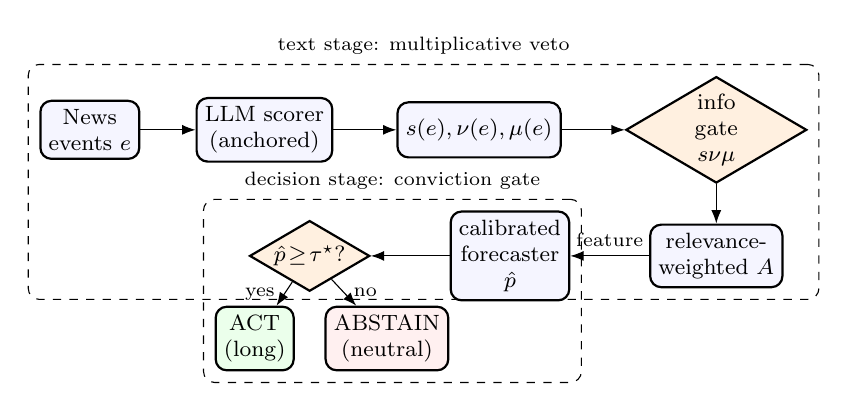
\begin{tikzpicture}[
  font=\footnotesize,
  box/.style={rectangle,rounded corners,draw,thick,align=center,inner sep=3pt,minimum height=7mm,fill=blue!4},
  gate/.style={diamond,draw,thick,align=center,inner sep=1pt,aspect=1.7,fill=orange!12},
  act/.style={rectangle,rounded corners,draw,thick,align=center,inner sep=3pt,fill=green!8},
  ab/.style={rectangle,rounded corners,draw,thick,align=center,inner sep=3pt,fill=red!6},
  >=Latex
]
\node[box] (text) {News\\events $e$};
\node[box,right=7mm of text] (llm) {LLM scorer\\(anchored)};
\node[box,right=8mm of llm] (dec) {$s(e),\nu(e),\mu(e)$};
\node[gate,right=8mm of dec] (g1) {info\\gate\\$s\nu\mu$};
\node[box,below=5mm of g1] (agg) {relevance-\\weighted $A$};
\node[box,left=10mm of agg] (model) {calibrated\\forecaster\\$\hat p$};
\node[gate,left=10mm of model] (g2) {$\hat p\!\ge\!\tau^\star$?};
\node[act,below left=4mm and -2mm of g2] (yes) {ACT\\(long)};
\node[ab,below right=4mm and -2mm of g2] (no) {ABSTAIN\\(neutral)};
\draw[->] (text)--(llm);
\draw[->] (llm)--(dec);
\draw[->] (dec)--(g1);
\draw[->] (g1)--(agg);
\draw[->] (agg)--(model) node[midway,above,font=\scriptsize]{feature};
\draw[->] (model)--(g2);
\draw[->] (g2)-- node[left,font=\scriptsize]{yes} (yes);
\draw[->] (g2)-- node[right,font=\scriptsize]{no} (no);
\begin{scope}[on background layer]
\node[draw,dashed,rounded corners,fit=(text)(g1)(agg),inner sep=4pt,label=above:{\scriptsize text stage: multiplicative veto}] {};
\node[draw,dashed,rounded corners,fit=(model)(g2)(yes)(no),inner sep=4pt,label=above:{\scriptsize decision stage: conviction gate}] {};
\end{scope}
\end{tikzpicture}
\end{document}
